%! program = pdflatex

\documentclass[11pt]{report}
\usepackage{geometry}
\geometry{a4paper}
\usepackage[parfill]{parskip}
\usepackage{fancyvrb}
\usepackage[T1]{fontenc}
\usepackage{graphicx}
\usepackage{amssymb}
\usepackage{epstopdf}
\usepackage{framed}
\usepackage{float}
\usepackage{color}

\sloppy

\usepackage[colorlinks=true, pdfstartview=FitV, linkcolor=blue,
            citecolor=blue, urlcolor=blue]{hyperref}

\setlength{\parindent}{0pt}
\setlength{\parskip}{2ex plus 0.5ex minus 0.2ex}

\title{Introduction to Access Management \\
using Oracle Access Manager}
\author{Horst Kapfenberger - Agora Con GmbH}
\date{May 10, 2016}

\begin{document}

\RecustomVerbatimEnvironment
  {Verbatim}{Verbatim}
  {numbers=left,frame=lines,fontsize=\scriptsize,framesep=4mm}


\maketitle

\begin{abstract}
    Introduction to Access Management in the area of Information
    Technology.  Description of user authentication, authentication
    factors and methods.
   
    Further explanation is done on the basis of an established
    proprietary software, \emph{Oracle Access Management Access
    Manager}.
    
    Detailed description of the Single-Sign-On process and the
    implementation in the considered product.

    Sample messages and software configuration excerpts are added.
\end{abstract}


\tableofcontents

% -----------------------------------------------------------

\chapter{Access Management}

\section{Prelude}

In \emph{Information Technology} the topic \emph{Access Management}
describes endeavours of managing user access to data and system
features.\footnote{User access:  beside human users other \emph{actors}
do exist.  Automated processes, sensors, interfaces or batch jobs
interact the same way.  We use the term user as comprehensive form of
actor, which implies \emph{including} all forms of access.} The sibling
discipline \emph{Identity Management}, delivers input to Access
Management --- a perpetually changing data set, containing user
identities and roles. All decisions are finally based on this set.

Access Management shall distinguish between the \emph{good ones} and the
\emph{bad ones}.  The good ones (users allowed to access) shall be
enabled to access business transactions without undesired limitations in
terms of time, location or device used. The supplementary effort needed
to get access shall be minimized.  As a consequence productivity will
increase.

The other group, the bad ones, are those we do not want to access the
system. No matter what efforts they undertake to get access,
unauthorized use shall be prevented and misuse shall be identified and
reported.

Access Management delivers sustainability in those areas:

\begin{description}

    \item[Application Security] --- restrict users and programs, recognise
        system abuse, identify identity theft
    \item[User Productivity] --- providing users with ease access to their
        needs, exactly to their needs: not more, not less
    \item[Middleware technology] --- save investments with process
        centralization and software reuse, providing interfaces based
        on open internet protocols
    \item[Compliance] --- as additional value delivered, compliance itself
        usually won't work as impulse or driver

\end{description}




\section{In Real Life: Border Controls}

A good comparison to illustrate the main characteristics of
authentication is \emph{border control}. That one you'll most often find
on airports or on the actual boarder between countries.\footnote{There
    was a time you had to leave \emph{Schengen Area} to find this seldom
experience, nowadays there seems to be an inflation of borderline
checks.}

You leave one domain, or more important: you enter another domain. 
A domain that has a certain definition, borders, and authorities that 
execute policies (for good and for bad, however).  Those brave officers 
want you to identify yourself --- your job is to provide them data, exact 
and distinct data and some prove that you tell the truth.

The data is usually good enough to identify you among all human beings.
That quality of your prove must satisfy the procedure of those border
checks. With a valid passport you own a document from a common trusted
authority that covers this.

\begin{enumerate}

    \item identifying you among all others \emph{(identification)} and
    \item prove the correctness of your statement
        \emph{(authentication)}

\end{enumerate}

For you, as the traveler, the desired outcome of this procedure is your
valid entry without much delay.


\subsection{Alternative Flows}

Thinking more general, what other situations in or outcomes of this
situation are possible?

\begin{itemize}

    \item you could pretend to be another person, perhaps from another 
        country
    \item you could sneak in the country, preventing any check
    \item you could mix you passport by mistake in the cafeteria next 
        to the borderline.  You enter the country with a different identity 
        without knowing
    \item your passport is expired and you are not allowed to enter the 
        country
    \item etc.

\end{itemize}

All those situations have a direct mapping to use cases in the IT world.


\subsection{Not Authorized}

One more thing is in common: at border controls there is no check what
exactly you are allowed to do --- in the country or domain.

There might be a rough categorization implied during the authentication,
like people with a certain nationality would need a visa or people out
of a certain country are not allowed to enter at all.

But this is not the place where a work or residence permit would be
checked.\footnote{At least as far the author knows.}

Using our vocabulary, we are \emph{authenticated} but no authorization
check has been done.

% -------------------------------------------------------------------

\chapter{Authentication}

\section{What's Authentication}

\emph{Authentication} is the act of confirming the truth of an attribute
of a single piece of data (a datum) claimed true by an entity. In
contrast with \emph{identification} which refers to the act of stating
or otherwise indicating a claim purportedly attesting to a person or
thing's identity, authentication is the process of actually confirming
that identity.


\section{Authentication Factors}

The ways in which someone may be authenticated fall into three
categories, based on what are known as the factors of authentication:
something the user \emph{knows}, something the user \emph{has}, and
something the user \emph{is}.

Each authentication factor covers a range of elements used to
authenticate or verify a person's identity prior to being granted
access, approving a transaction request, signing a document or other
work product, granting authority to others, and establishing a chain of
authority.


The three factor types and some of elements of each factor are:

\begin{description}

    \item[Knowledge Factor] Something the user knows --- e.g.\ a 
        password, Partial Password, pass phrase, or personal identification 
        number (PIN), challenge response (the user must answer a question, 
        or pattern), Security question

    \item[Ownership Factor] Something the user has --- e.g.\ wrist band, 
        ID card, security token, cell phone with built-in hardware token, 
        software token, or cell phone holding a software token

    \item[Inherence Factor] Something the user is or does --- e.g.\ 
        fingerprint, retinal pattern, DNA sequence (there are assorted 
        definitions of what is sufficient), signature, face, voice, 
        unique bio-electric signals, or other biometric identifier

\end{description}


For authentication to well-secured systems elements from at least two,
and preferably all three, factors should be verified.


\section{Authentication Methods}

What information the user is requested to enter during authentication
and how this information is passed to the service, this is defined as
authentication method.

Authentication methods are standardized, usually in RFC, to enable
interoperability and to ensure a certain system security among different
implementations.  Authentication is a critical process and is target to
all kinds of security attacks.

\begin{description}

    \item[User Passwords] \emph{Knowledge factor.}  The most common used
        method is also considered as the weakest and most problematic
        one.  Users seem to be very bad in \emph{choosing} password, in
        \emph{remembering} them and in \emph{changing} them
        periodically.\footnote{To increment an included number is not
        considered as proper password change.}
            
        Another risk is the transport of the real password over the
        wire, what is the typical implementation in web
        applications.\footnote{Mail clients offer alternative, standard
        transport methods for over a decade now.}
        
        On the other hand application developers seem to be good in
        creating unsecure implementations, especially in storing or
        dealing with passwords. Bottom line: if possible, prevent using
        passwords in general.
    
    \item[Kerberos] \emph{Knowledge and ownership factor.}  Kerberos is
        a distributed ticketing system, passing encrypted keys a
        credentials. Kerberos version 5 is included in every mainstream
        Unix/Linux/BSD system and Microsoft Windows as the default
        authentication method.
        
        Kerberos is the preferred method of authentication within LAN
        network, but it was not widely used on WAN because an additional
        communication port would have been necessary. With MS-KKDCP from
        Microsoft this seems to change, it has been adopted by many open
        source groups and vendors.
        
    \item[RSA Token] \emph{Knowledge and ownership factor.}  Proprietary
        implementation from RSA Security Inc., currently a division of
        EMC Corporation. Often used in Enterprise VPN solutions. RSA is
        known to distribute products with backdoor for security
        services.  Especially problematic are RSA libraries included in
        3rd party products (e.g.\ Dual\_EC\_DRBG in Windows, Java,
        OpenSSL).

        While its not recommended to use RSA Token, several alternatives
        do exist that are considered secure, some of them are internet
        standards.\footnote{RFC 1760 (S/KEY), RFC 2289 (OTP), RFC 4226
        (HOTP) and RFC 6238 (TOTP).} More user-friendly then hardware
        tokens are software versions for mobile devices, providing multi-
        service-provider support.

    \item[Client Certificates] \emph{Knowledge and ownership factor.}
        X.509 certificates are considered to be secure. Prerequisite is
        a private key infrastructure (PKI) with an online revocation
        service though. Client certificates are often used within an
        organization with an independent, self-signed certification
        authority. This requirement makes it difficult (or too
        expensive) for global usage. This might change in the near
        future, as changes in the CA business model are already taking
        place.

\end{description}


            
% -------------------------------------------------------------------


\chapter{Access Management Suite}

\section{Suite Overview}

Around 2010 Oracle corporation acquiree a dozen software vendors and
technology companies in the identity and access management market. Among
them were some niche players and also leaders, like Sun Microsystems
with several active products and a stable user base.

Developing a portfolio of twenty specialized systems to two or three
tightly integrated solutions definitely the overall plan, but not every
step is set straight on that path, looking at the footsteps we see
sometimes.

Next to the Identity Management Suite the Access Management Suite is the
second major product group, where the collected technologies deal with
run-time evaluation of user or system access.

The Access Manager itself is the heart of Suite, where other products or
new feature sets have been integrated or merged into.

\begin{itemize}
    \item Access Manager
    \item Identity Federation
    \item Security Token Service
    \item Mobile and Social
    \item Adaptive Authentication Service
    \item OAuth Services
    \item Identity Context
\end{itemize}



\section{Suite Applications}


\subsection{Access Management Access Manager}

As the central part of the suite, Access Manager delivers the
administrative user interface. All authentication mechanisms are defined
here and components and processes can be activated or cut-off in the
admin user interface. Business applications can be registered and
external data sources containing identity data may be connected.

Distributed components, the policy enforcement points, are located
closer to the protected business applications and request authentication
and authorization information from the central access server over
encrypted channels.


\subsection{Identity Federation}

While Access Manager takes care of a single domain (or multiple but
independent domains), Identity Federation helps to connect domains
(e.g.\ two organizations with integrated business activities).  In each
activity the roles and responsibilities are well defined. Identity
Federations supports SAML and OpenID\@.


\subsection{Security Token Service}

Token validation and generation to facilitate access to services across
security domains and beyond organizational boundaries. Essentially the
service acts as a trust-broker that receives and validates client
requests and generates appropriate tokens for a requested resource.


\subsection{Mobile and Social}

Mobile (for mobile devices): integrate iOS and Android mobile devices,
policy enforcement on those devices, single-sign-on for mobile apps and
browser based access, SDK on mobile devices.

Social (for social services): integrate authentication, policies for
several social services available on Internet.


\subsection{Adaptive Authentication Service}

Real-time and batch risk analytics to prevent fraud and misuse, risk
based authentication, additional authentication methods, like
One-Time-Passwords (OTP).


\subsection{OAuth Services}

OAuth 2.0 authentication client and server. Manage access control over
domain borders.


\subsection{Identity Context}

Enable dynamic adaption of permissions based on user related data, like
location, last transactions, third party informations, other assigned
permissions, etc.


This document covers topics from Access Management Access Manager only.


% --------------------------------------------------------------------

\chapter{Access Manager}


\section{Overview}

The role of Access Manager can be described as a gate keeper, in front
of all business applications. Each user request needs to pass this gate
keeper. It ensures that only authenticated requests are allowed to reach
the protected business application.

\begin{framed}

    All integration practices described are considering the integration
    of web applications. Web applications are applications that deliver 
    the user interface via HTTP or HTTPS\@.

\end{framed}

Access Manager delivers a common used, central login functionality, the
user authentication. The authentication method presented to the user is
determined based on several input parameter, like the resource the user
tries to access, the date and time, perhaps the user location or device
used, or the type of user access manager recognizes already
before the authentication.

The implementation of login functionality is per se critical and it is
critical in multiple ways:

\begin{itemize}

    \item run time errors may block the whole business application

    \item often an external system call is needed, the response data 
        and its interpretation is not obvious or may change over time

    \item accounts may be locked in different ways, what shall be the 
        user error message?

    \item the business application (perhaps a closed source 3rd party
        application) needs to deal with user passwords

\end{itemize}

Dealing with all those challenges, a centralized solution like a
directory server, feels again like a redundant and error prone approach.
Quite often it also becomes a dangerous approach, when one of the
business applications or an operational tool is lacking the latest and
mandatory encryption cipher and now sends plain text or it logs one
attribute more than it should (yes, credentials in log files is not an
uncommon problem).


But not all application areas may trigger an authentication.  For public
accessible areas the authentication check can be disabled in the
\emph{application domain} configuration. In addition auditing records
can be disabled for public accessible area.  This prevents data
collections of no usage or even prohibited usage.

The single-sign-on session of an authenticated user includes its current
authentication level.  We can perceive the session as an \emph{ticket}
to the systems behind the gate keeper.  This ticket is stored central on
the access server and also on the client (using cookies, protected
against external changes). This authentication level is matched the
minimum authentication level attached to the resource the user requests.

The boundaries of the single-sign-on session can be defined by domain
and subdomain namespaces. However this will only be enforced for
integrated applications.

Each session has set a \emph{general time-out} and an \emph{inactivity
time-out}. The general time out will close the session and force a
re-authentication, no matter if there is currently any activity ongoing
or not. Default value of this general time-out is 24 hours. The
inactivity time-out is set to a shorter period, depending on the
customer needs and security level.


\section{Application Integration}

Business applications often require an independent application session,
where user data is attached to. This session information is not touched
by Access Manager.

Before our integration, the business application did act a as a
stand-alone application, in terms of the user session. An application
login page was presented to the user, in case the user had no active
session.

The \emph{integration} of an application is relative simple exercise,
since we essentially remove functionality and code. In particular the
login and logout functionality is removed. Instead of returning an
application login page, the application can take the attached
information like user name, user ID, or roles, and continue with the
transaction.

The logout link or button of the business application will remain on the
user interface. The business application will just redirect the user to
the general logout URI, which will trigger the necessary logout
callbacks to the used business applications. So the user sessions will
safely be closed on a general logout. However, as before this is
triggered when the user actively executes a logout.

The individual implementations of the user login and logout are removed
from applications during integration. Only authenticated requests can
reach the application from now on. While an authorization policy
enforcement is available and recommended, other products of the suite
may be necessary to cover different authorization requirements.



% ====================================================================

\chapter{Components of Access Manager}

In the following pages I will explain what parts or topics Access
Manager consists of and what the are good for:

\begin{itemize}
    \item Access Server
    \item Application Domains and Resources
    \item Identity Store
    \item Session Store
    \item Policy Enforcement Points: Agents
    \item Webgate Agent
    \item SSO Cookies
    \item Credential Collector
    \item Certificate Validation and Revocation
\end{itemize}




\section{Access Server}

The Access Server is the \emph{backend runtime component} that serves
requests of the \emph{Policy Enforcement Points}. It is implemented as
J2EE service and Oracle supports Oracle WebLogic and IBM WebSphere as
application servers. In WebLogic the services are deployed to one or
more managed servers grouped in a WebLogic cluster.  Most of the
interfaces and protocols are based on open standards, an exception here
is the proprietary protocol to the policy enforcement points, called OAP
(Oracle Access Protocol).

The configuration can be done using the web user interface 
\emph{OAMConsole}, hosted on the WebLogic Admin Server. Many features
can also be configured using shell scripts or the WebLogic scripting
environment WLST\@. The substantial configuration is persisted as XML
file. Bindings and policies are stored in the relational database base
schema.


\section{Application Domains and Resources}

The value of an production access system, comes from the integrated
business applications. Therefore the management of those business
applications and their policies is a central area in Access Manager.

Applications are mapped to application domains. This mapping can be done  
as an one-to-one relation, but also other transformations are possible,
as long as it helps the operational team to treat the integration as one
consistent block of applications, which is integrated or maintained at
once.

Each application domain consists of multiple resources. A resource can
be seen as an entitlement in the application domain. Since all resources
are expressed as \emph{Uniform Resource Identifier (URI)}, Access
Management uses the URI component \emph{path} and optionally \emph{query} and
\emph{fragment} as resource identifier.

Example resource identifier: \verb|/orders/**|



\section{Identity Store}

To execute the main feature of Access Manager, the authentication, we
need at least one set of identities that are allowed to authenticate.
This set must be stored in a supported directory server and should be
\emph{close} to Access Manager, in operational and data ownership
perspective.

Access Manager will read from and write to this identity store. The
required initial information in the store is the user login and some
status information of the user account.

Access Manager stores additional runtime data attached to the user
information.

Optional information that can be stored in the identity store can be
\emph{user credentials}, \emph{user roles}, etc.

In case you deploy \emph{Access Manager} with \emph{Oracle Identity
Manager} the directory is automatically populated and acts as a data hub
between Identity and Access Management.


\section{Session Store}

We already mentioned where user sessions are stored. But let's have a
closer look here.

For Access Manager it is essential to have clear accounting of active
user sessions, with additional information attached to them:

\begin{itemize}
    \item when did the session start
    \item timestamps used for time-outs
    \item authentication method used
    \item current and original authentication levels
    \item reference to identity store
    \item location (if applicable)
\end{itemize}

This information must be served quickly with high availability
requirements. Access Manager maintains this list in Coherence.

\begin{framed}

    Oracle Coherence is a proprietary in-memory data grid, that improves
    performance, scalability and reliability compared to relational
    databases. It can be used as an persistence system or as a caching
    method in combination to relational database system.
    
    Coherence was developed by \emph{Tangosol Inc.}, which was acquired 
    by Oracle Corporation in 2007. Several Oracle applications, like 
    Access Manager or SOA, use Coherence.

\end{framed}

The Access Manager admin interface \emph{oamconsole} comes with a
feature for querying and maintaining the session list.

The session information placed at the client side is described in the
section Cookies.


\section{Policy Enforcement Points: Agents}

The Policy Enforcement Points (PEP) are the components actively asking
Access Manager for user access and are enforcing this policy. They act
as gatekeeper to the business applications. One agent implementation is
shipped with the Access Manager Suite, other Oracle implementations are
available but are considered deprecated. Furthermore individual
implementations are supported.

To fulfill its work as gatekeeper a PEP has to be involved in every
client request to the business application, preferably very early in the
request processing to protect the application from different types of
attacks.

For web applications this is usually done in the \emph{demilitarized zone
(DMZ)}, on an perhaps already existing \emph{reverse proxy}.

For incoming request those attributes are evaluated:

\begin{itemize}
    \item requested resource (URI): host and path
    \item existing cookies
    \item misc.\ attributes, like location, etc.
    \item verification data from access server
\end{itemize}

Since there is no policy information stored in distributed locations,
where PEP are deployed, those information must be gathered from the
access server.  This information is heavily cached in the PEP, to speed
up decision response time and throughput.

Possible outcomes of the decision are:

\begin{itemize}
    \item redirect to credential collector
    \item let request pass with audit entry
    \item let request pass without audit entry
\end{itemize}

The communication to the Access Server is crucial and must be protected
against attacks. Access Manager and the PEP implementation can be
configured to use a general encryption key (this is the default setting)
or agent instance related keys.


\section{Webgate Agent}

The Webgate Agent is a Policy Enforcement Point implementation to deploy
on HTTP Servers like \emph{Oracle Web Server} or the \emph{Apache
HTTPD}.\footnote{There has been a version available for Microsoft
    Internet Information Server (IIS). This versions was seemed to be outdated
    and the author was not able to install this binary successfully.
    Since reverse proxies based on Windows are not widely used, I would
not expect further development in this area.} It is shipped as a binary,
compiled for the main platforms, and is integrated as a module for the
web server. No additional run time process is necessary.

The necessary configuration is done inside the HTTPD configuration file
and a general setup with its own configuration file. The communication
channel to the Access Server is protected by certificates located in
configuration directory. There are two types of protection:

\begin{itemize}
    \item protecting all agents with the same key
    \item protecting each agent with an individual key
\end{itemize}

The standard HTTPD configuration defines which requests are covered by
Webgate.  For not included resources Webgate and Access Manager are not
involved at all.  For covered resources the decision outcome may also be
\emph{public available}, however the resource must be known to Access
Manager, otherwise an error will be returned to the user.

Agents can be configured with a broad range of log options. Those logs
are stored on the reverse proxy and are not to be confused with the
central stored audit logs. Particular care is recommended to not include 
sensitive request payload information in the log files.


\section{SSO Cookies}

Within the area of Access Manager nine different types of HTTP cookies
are used. Typically three or four cookies are in use in one setup,
if legacy support is needed. Those cookies are automatically encrypted
or signed by the server components.

The \emph{Oracle Fusion Middleware Administrator's Guide for Oracle Access
Management} contains the exhausted list of nine types and description
under what circumstances each type is deployed.



\section{Credential Collectors}

Credential Collectors are web sites with an embedded form, requesting a
user identifier and  credentials to authenticate. The user is redirected
to a credential collector, because he requested a resource and his
current authentication level is lower than required for accessing the
requested resource. To access the resource an certain authentication is
necessary and the user is required to do so. During the authentication
process the original request shall not be lost, otherwise the user would
perhaps authenticate successfully but not get the resource he asked for.
Therefore the request data is dragged along the whole process.

There are two types of credential collectors:

\begin{description}

    \item[Embedded Credential Collector (ECC)] Located in 
        WebLogic managed server of Access Manager. The ECC is shipped
        with the product, customization possibilities are limited.

    \item[Detached Credential Collector (DCC)] Located outside 
        Access Manager, preferably in the DMZ\@. No Java application
        server needed. A \emph{Perl} implementation as sample code is 
        included with product.

\end{description}

The main difference is the location in the network architecture and the
security consequences of this decision. While the usage of ECC allow 
unauthenticated requests to reach application tier, DCC terminates all
unauthenticated requests already in the DMZ\@. 



\section{Certificate Validation and Revocation}

This module delivers standard services for a \emph{Private Key
Infrastructure (PKI)} for announcing the validity of X.509 certificates
in a domain. The current version of the service definition can be found
in 

\begin{itemize}

    \item RFC 5280 Internet X.509 Public Key Infrastructure Certificate
        and Certificate Revocation List (CRL) Profile

    \item RFC 6960 X.509 Internet Public Key Infrastructure Online
        Certificate Status Protocol (OCSP)

\end{itemize}

While CRL are signed list of all certificate revocations of the domain,
OCSP is an online status protocol that can be used by clients or 
during preprocessing by a delivery service, know as \emph{OCSP Stapling}.


% -------------------------------------------------------------------------


\chapter{Requested Feature Descriptions}


\section{Authorization Policies}


Access Manager offers an additional security layer for protecting resources,
After evaluating the authentication policy attached to a resource, Access
Manager looks for an existing authorization policy.  Authorization policies can
narrow the set of users allowed to access a certain feature.  

\begin{description}

    \item{Example 1}: The admin features of a sales application shall only be
        accessible from the internal network and only during business hours.

    \item{Example 2}: The order cancellation feature shall only be accessible by
        user authenticated by Kerberos or RSA Token.

\end{description}

Authorization policies in Access Manager are not meant to be a replacement for
the typical authorization features within a business application. As an
additional protection layer in front of the business application, the main
benefits are:

\begin{itemize}

    \item Additional line of protection of sensible features, like
        administrative user interfaces or whole business applications. Without
        Access Manager a single mistake in the business application would
        expose critical transactions or data to unauthorized users.

    \item Common configuration and reporting over all applications. Without
        Access Manager multiple sources or departments need to be consulted.

    \item Enable new levels of security: access can be granted based on the
        quality of the authentication method. Additional authentication steps
        (e.g.\ transaction codes or hardware tokens) may enable user to execute
        additional transactions or increase certain thresholds.

    \item Authorization based on user location (IP address) or within defined
        time frame is possible.

\end{itemize}


\subsection{Implementing Authorization Policies}

Authorization policies are defined in an application domain and are attached
resources of the domain --- like authentication policies.

Authorization policies consist of conditions, rules and responses.  The
evaluation of the policy shall deliver a boolean result value --- allow or deny
--- and an optional response value.


\begin{description}

    \item{Rules} --- rules are executed to get the boolean return value true
        (allow) or false (deny). Not returning any value is not allowed.  Rules
        consist of conditions.

    \item{Conditions} --- conditions are user or environment attribute
        comparisons.  See below for details.

    \item{Responses} --- are the result values of the policy can be exported
        for reuse within Access Manager or for the business application. The
        result can be attached to the request (as HTTP header variable), to the
        session or to the cookie.

\end{description}


\subsubsection{Conditions}

For expressing the rules there are four types of conditions available. However
it's not the condition that renders allow or deny --- the interpretation of the
condition result is done in the rule.


\begin{description}

    \item{Identity} --- Makes use of Access Managers identity stores in two
        possible ways. One is the static definition of a set of identities from
        the identity store. The other is to express LDAP queries against the
        store.

    \item{IPv4 Address Range} --- The interpretation of client IP address
        ranges depends on your user base. Usually important information about
        the client can be derived from the IP address. Currently only IPv4 is
        supported.

    \item{Temporal} --- Time periods, expressed as day of the week, from HH:MM
        and to HH:MM\@.  The time entered here is always evaluated as Greenwich
        Mean Time (GMT) without any adjustment of possible daylight savings
        time.

    \item{Attribute} --- attributes that are attached to the user request, the
        session, or the user LDAP object can be used in the comparison. Among
        them are session count, authentication scheme or level, resource name
        or host name,

\end{description}


% -------------------------------------------------------------------------

\chapter{Proof of Concept}

\section{Summary}

The Proof of Concept (PoC) is virtual machine including all software and
configuration to run \emph{Oracle Access Manager 11gR2} and an additional web
application that has been integrated into the Access Manager architecture.

The Oracle components have been setup automatically using \emph{iam-deployer}.
The project management software \emph{Redmine} is used to demonstrate the
integration procedure and Access Manager features.


\section{Software Components}

The virtual machine is running CentOS 6.7 64bit, 32 GB RAM and a total
disk space of 50 GB have been assigned.  For kernel parameter and system
configuration please see \emph{iam-deployer}.

Following Oracle suite components are setup:

\begin{itemize}

    \item Oracle Access Manager 11.1.2.3
    \item Oracle Identity Manager 11.1.2.3
    \item Oracle Unified Directory 11.1.2.3
    \item Oracle HTTP Server 11.1.2.3 (based on Apache 2.2) 
    \item Oracle Database Enterprise Edition 11.2

\end{itemize}

The sample web application consists of these components:

\begin{itemize}

    \item Redmine 3.2.1
    \item Thin 1.6.4 (Ruby 2.3, Rails 4.2)
    \item MySQL Server 5.1.73

\end{itemize}

Hardware load balancer replacement and TLS termination:

\begin{itemize}

    \item HAProxy 1.5.4

\end{itemize}


Since PS3 the default setup of the Oracle suite requires an amount of RAM that
makes it difficult to run the virtual machine on a standard laptop.  Therefore
the VM is hosted in Vienna, access for DWP Bank is enabled.  An copy of the VM
can be downloaded.



\section{SSO Process Flow}

A sign-on using Access Manager triggers a certain number of system
interactions, depending on the configuration, the requested resource and the
required authentication methods.

The first diagram is a simplified overview, the second is a more detailed
sequence diagram of those interactions.


\begin{figure}[H]
    \centering
    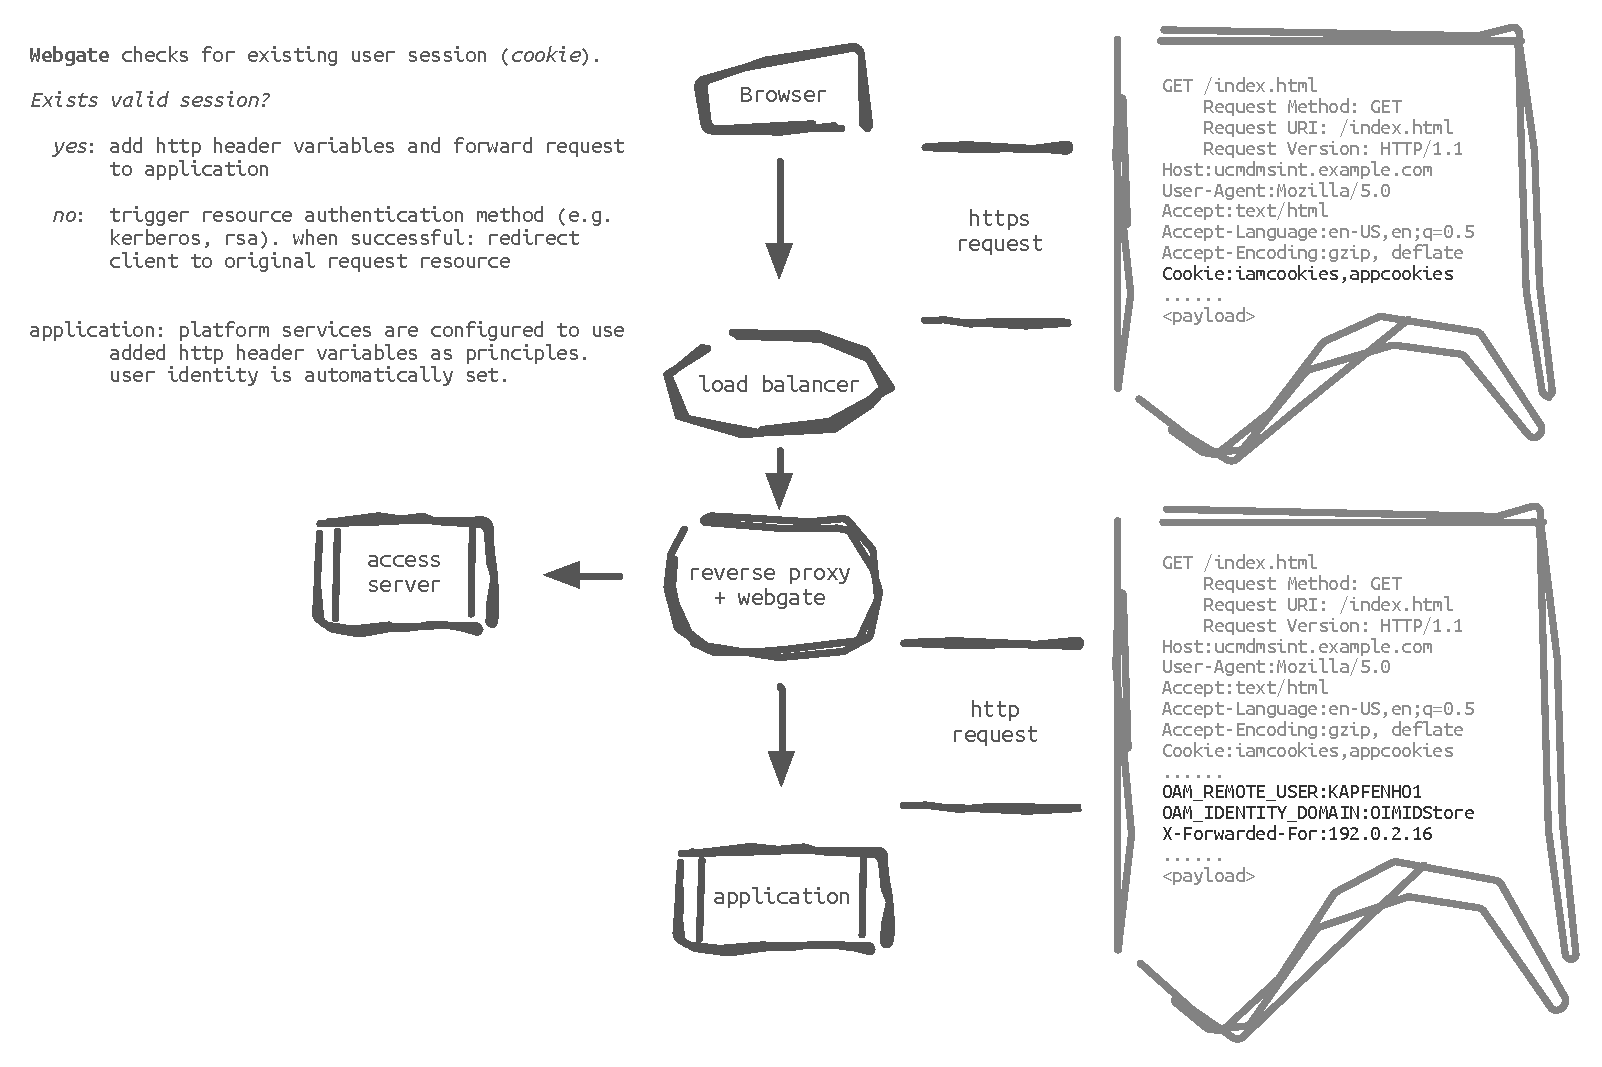
\includegraphics[width=1\textwidth]{diag/msgdiag}
    \caption{Login process with messages}
\end{figure}


\begin{figure}[H]
    \centering
    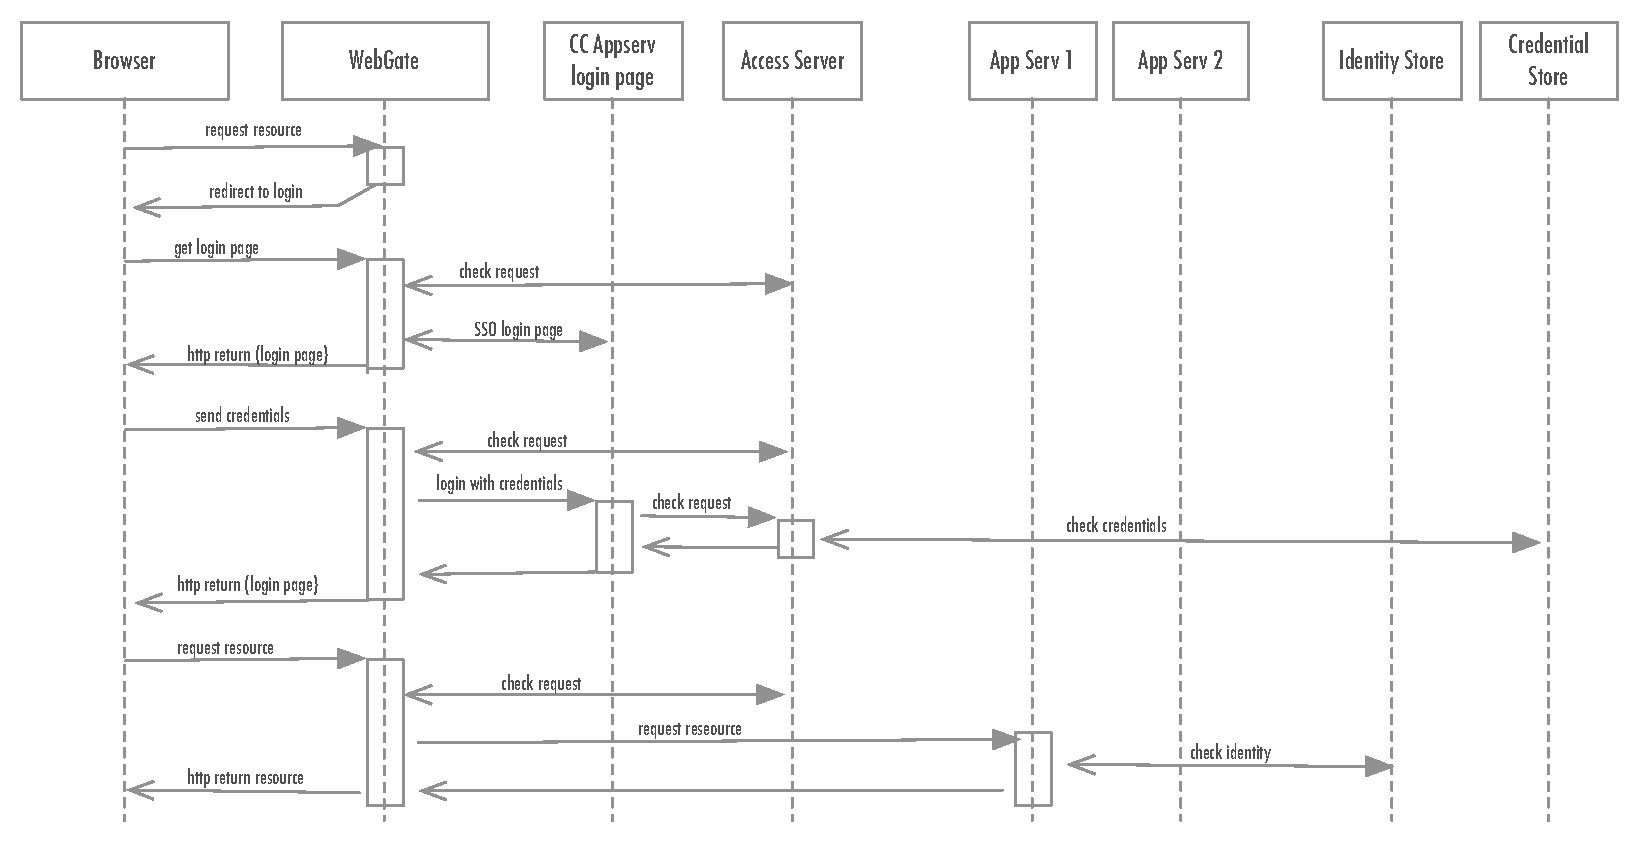
\includegraphics[width=1\textwidth]{diag/seqdiag}
    \caption{Sequence diagram of SSO login process}
\end{figure}



\section{HTTP Routing}

It is important to understand the routing of the client HTTP requests.  The
access control is taking place before the request reaches the addressed
resource.

\begin{figure}[H]
    \centering
    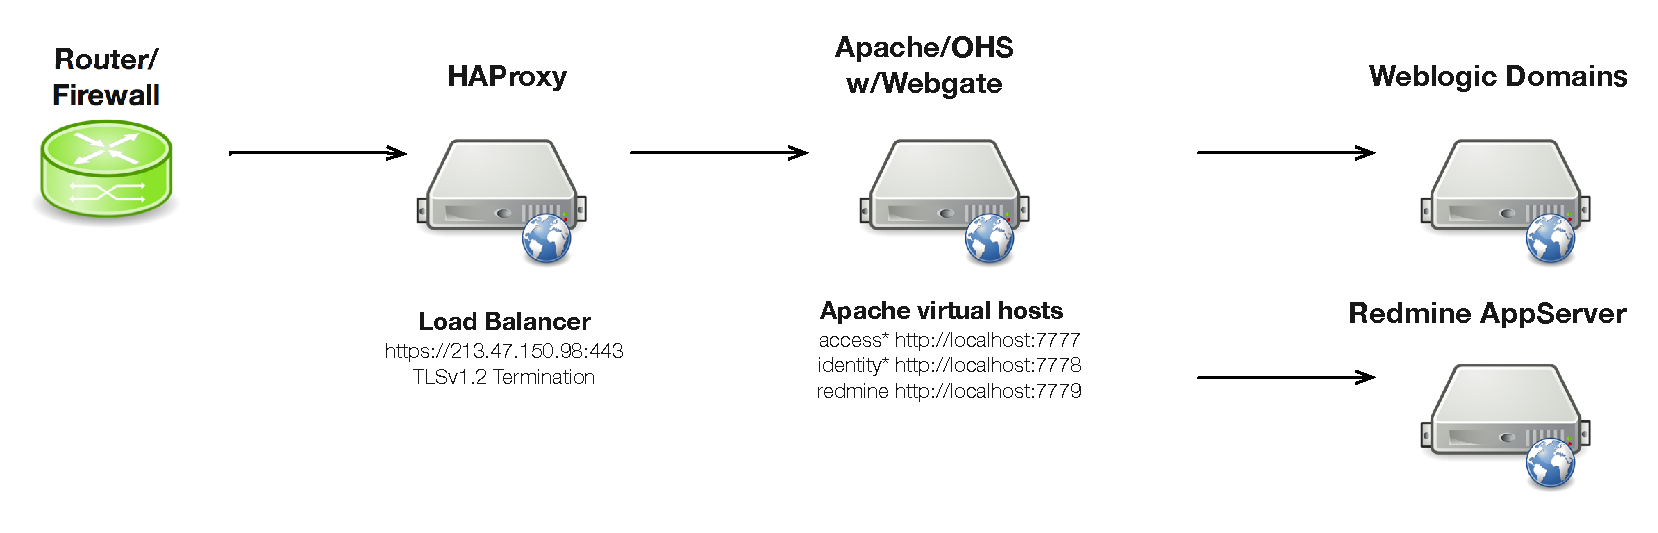
\includegraphics[width=1\textwidth]{diag/iamvs}
    \caption{HTTP routing to applications}
\end{figure}


\newpage

\section{Infrastructure Configuration}

The configuration here is based on an properly configured Access Manager
instance, e.g.\ created by \verb|iam-deployer|.


\subsection{Domain Name Entries}

The Oracle applications and the new webapp are accessed using different host
names.  This is not mandatory but a recommended approach for putting several
applications on one access point.

This \emph{domain name entries} have been configured for the instance:


\begin{Verbatim}[label=DNS Zone]
$ORIGIN agoracon.at.
$TTL 86400 
@               86400   IN    SOA       dns1.agoracon.at. admin.agoracon.at. ( 
                                            2016042013  1d 1h 4w 1h )

...

iamvs                   IN    A         213.47.150.108
                        IN    TXT       "v=SUB access identity redmine"
access.iamvs            IN    CNAME     iamvs
access-admin.iamvs      IN    CNAME     iamvs
access-api.iamvs        IN    CNAME     iamvs
access-mobile.iamvs     IN    CNAME     iamvs
identity.iamvs          IN    CNAME     iamvs
identity-admin.iamvs    IN    CNAME     iamvs
identity-api.iamvs      IN    CNAME     iamvs
dir-admin.iamvs         IN    CNAME     iamvs
omsas.iamvs             IN    CNAME     iamvs
redmine.iamvs           IN    CNAME     iamvs
...

_443._tcp.iamvs.agoracon.at. 86400 IN TLSA (1 0 1 fingerprint...)
...
\end{Verbatim}


Recommended security mechanisms:

\begin{itemize}

    \item DANE\footnote{RFC 6394: Use Cases and Requirements for DNS-Based 
	Authentication of Named Entities (DANE)} and TLSA\footnote{RFC 6698: 
	The DNS-Based Authentication of Named Entities (DANE) Transport 
	Layer Security (TLS) Protocol: TLSA}

    \item HTTP Strict Transport Security\footnote{RFC 6797: HTTP Strict 
	Transport Security (HSTS)}

    \item DNSSEC\footnote{Around a dozen RFC and growing. A good start point 
	is RFC 4033: DNS Security Introduction and Requirements}

\end{itemize}


\subsection{Load Balancer}

A software replacement for the hardware load balancer used in production is
configured in the virtual machine.  This enables operations to use the same web
configuration across all environments.  \verb|HAProxy| can be installed as an
OS repository package.

The configuration used for this instance:

    \begin{Verbatim}[label=haproxy.conf]
#  $haproxy: haproxy.conf,v 1.0 2016/04/06 16:25:44 kapfenho Exp $
#  vi:ft=haproxy:
#  Part of IAM deployment
#
global
    daemon
    log         127.0.0.1 local2
    chroot      /var/lib/haproxy
    pidfile     /var/run/haproxy.pid
    maxconn     4000
    user        haproxy
    group       haproxy
    stats socket /var/lib/haproxy/stats
    # tuning
    tune.ssl.default-dh-param 2048
    tune.ssl.cachesize 20000
    tune.ssl.lifetime 3600

defaults
    mode      http
    log       global
    option    httplog
    option    dontlognull
    option    http-server-close
    option    forwardfor       except 127.0.0.0/8
    option    redispatch
    retries   3
    timeout   http-request    10s
    timeout   queue           1m
    timeout   connect         10s
    timeout   client          1m
    timeout   server          1m
    timeout   http-keep-alive 10s
    timeout   check           10s
    maxconn                 3000


frontend  http_proxy
    bind *:80
    redirect scheme https if !{ ssl_fc }

frontend  https_proxy
    bind *:443 ssl crt /etc/haproxy/x509/iamvs.pem force-tlsv12

    acl host_red hdr_beg(host) -i redmine
    acl host_oim hdr_beg(host) -i identity-api.
    acl host_oim hdr_beg(host) -i identity.

    default_backend oam
    use_backend red if host_red
    use_backend oim if host_oim

backend oam
    server oam1 localhost:7777 maxconn 256 check

backend oim
    server oim1 localhost:7778 maxconn 256 check

backend red
    server red1 localhost:7779 maxconn 256 check
\end{Verbatim}


\newpage

\section{Integration Tasks}

To integrate a web application into Access Manager the following tasks need to
be performed:

\begin{itemize}

    \item Place Policy Enforcement Point on request path (infrastructure)
    \item Configure Application Domain in Access Manager (Access Manager)
    \item Remove application login and configure SSO user (application)
    \item Change logout behaviour (application)

\end{itemize}

Changes in Access Manager can be done using the user interface
\emph{oamconsole}, by importing XML definition files or by using the WLST
scripting interface.


\subsection{Routing via Policy Enforcement Point}

A policy enforcement point (PEP, e.g.\ Webgate) needs to be able to inspect the
client request.  This can be achieved by using an already existing reverse proxy
with PEP, creating an additional reverse proxy with PEP or deploy Webgate to an
existing reverse proxy.  There are also some commercial firewall products
available, that contain compatible PEP (additional fees may apply for add-ons).\@

Additional PEP need to be registered in Access Manager.  The communication
between Access Manager and the PEP needs to be secured.  This can be done in a
general way for all PEP (of the same type) or by individual certificates for
each PEP instance.


\subsection{Configure Application Domain in Access Manager}

The new application domain can be configured using the user interface or by
definition import.  The domain definition contains all resource definitions 
along with their authentication and authorization policy. 

\begin{Verbatim}[label=Register Application Domain]
<?xml version="1.0" encoding="UTF-8"?>
<PolicyRegRequest>
    <serverAddress>http://iamvs.agoracon.at:7001</serverAddress>
    <hostIdentifier>iamvs.agoracon.at</hostIdentifier>
    <applicationDomainName>RedmineDomain</applicationDomainName>
    <protectedAuthnScheme>LDAPScheme</protectedAuthnScheme>
    <protectedResourcesList>
        <resource>/account/**</resource>
        <resource>/news/**</resource>
        <resource>/issues/**</resource>
        <resource>/projects/**</resource>
        <resource>/boards/**</resource>
        <resource>/journals/**</resource>
        <resource>/imports/**</resource>
        <resource>/my/**</resource>
        <resource>/users/**</resource>
        <resource>/wiki/**</resource>
        <resource>/time_entries/**</resource>
        <resource>/activity/**</resource>
        <resource>/attachment/**</resource>
        <resource>/groups/**</resource>
        <resource>/trackers/**</resource>
        <resource>/admin/**</resource>
        <resource>/workflows/**</resource>
        <resource>/**</resource>
    </protectedResourcesList>
    <publicResourcesList>
        <resource>/public/**</resource>
    </publicResourcesList>
    <excludedResourcesList>
        <resource>/excluded/**</resource>
    </excludedResourcesList>
    <hostPortVariationsList>
        <hostPortVariations>
            <host>redmine.iamvs.agoracon.at</host>
            <port>7779</port>
        </hostPortVariations>
    </hostPortVariationsList>
    <rregApplicationDomain>
    </rregApplicationDomain>
</PolicyRegRequest>
\end{Verbatim}


\subsection{Login Process Integration}

With the Access Manager integration the application won't need an login screen
on it's own any more.  Where ever an authentication is necessary, the request
will be authenticated before it reaches the application.  The application needs
to take the principal set by Access Manager.

In our example HTTP header variable named \verb|HTTP_OAM_REMOTE_USER| is used
for passing the user identifier.  Using header variables is common method for
SSO, commercial software products usually support this by configuration.

A customization for a Rails application is done with three additional lines
(including the comment).


\begin{Verbatim}[label=Changes for Login]
diff --git a/app/controllers/application_controller.rb b/app/controllers/application_controller.rb
index 092c83a..f8741a6 100644
--- a/app/controllers/application_controller.rb
+++ b/app/controllers/application_controller.rb
@@ -103,6 +103,9 @@ class ApplicationController < ActionController::Base
         user = (User.active.find(session[:user_id]) rescue nil)
       elsif autologin_user = try_to_autologin
         user = autologin_user
+      elsif request.env["HTTP_OAM_REMOTE_USER"]
+        # userid passed by oam in http header
+        user = (User.active.find_by_login(request.env["HTTP_OAM_REMOTE_USER"].to_s) rescue nil)
       elsif params[:format] == 'atom' && params[:key] && request.get? && accept_rss_auth?
         # RSS key authentication does not start a session
         user = User.find_by_rss_key(params[:key])
\end{Verbatim}



\subsection{Logout Process Integration}

The following lines are taken from a reverse proxy access log and show the SSO
logout process.  In this session two applications were used, Redmine and the
Access Manager oamadmin application.


\begin{Verbatim}[label=HTTP Calls during Logout]
     redmine.iamvs.agoracon.at "POST /logout                HTTP/1.1" 301 117
     redmine.iamvs.agoracon.at "GET  /oamsso/logout.html    HTTP/1.1" 302 261
      access.iamvs.agoracon.at "GET  /oam/server/logout     HTTP/1.1" 200 3111
     redmine.iamvs.agoracon.at "GET  /oam_logout_success    HTTP/1.1" 200 114
access-admin.iamvs.agoracon.at "GET  /oam_logout_success    HTTP/1.1" 200 114
      access.iamvs.agoracon.at "GET  /oam/pages/logout.jsp? HTTP/1.1" 200 1899
\end{Verbatim}


The POST with resource \verb|/logout| is taken by the agent and redirected to
the agent default logout page (\verb|/oamsso/logout.html|), followed by a call
to the access server central logout (\verb|/oam/server/logout|).  The session
information is invalidated now on server side (Coherence) and on client side
(Cookies).  A sequence of call-backs to applications involved in this session
is processed, triggering the application specific logouts
(\verb|/oam_logout_success|).  Eventually the user gets the configured post
logout page.


\begin{Verbatim}[label=Changes for Logout]
diff --git a/config/routes.rb b/config/routes.rb
index 9652496..bdaf675 100644
--- a/config/routes.rb
+++ b/config/routes.rb
@@ -19,7 +19,10 @@ Rails.application.routes.draw do
   root :to => 'welcome#index', :as => 'home'

   match 'login', :to => 'account#login', :as => 'signin', :via => [:get, :post]
-  match 'logout', :to => 'account#logout', :as => 'signout', :via => [:get, :post]
+  match 'logout' => redirect('/oamsso/logout.html'), as: :signout, via: [:get, :post]
+  match 'oam_logout_success', :to => 'account#logout', :via => [:get, :post]

   match 'account/register', :to => 'account#register', :via => [:get, :post], :as => 'register'
   match 'account/lost_password', :to => 'account#lost_password', :via => [:get, :post], :as => 'lost_password'
   match 'account/activate', :to => 'account#activate', :via => :get
\end{Verbatim}


% -------------------------------------------------------------------------

\chapter{Miscellanies}


\section{Authenticated Request}

An authenticated user requests a resource. Webgate has successfully verified the
request and added the user identifier (\verb|OAM_REMOTE_USER|) and domain
(\verb|OAM_IDENTITY_DOMAIN|). The request is now passed to the upstream system.

\begin{Verbatim}
Hypertext Transfer Protocol
    GET /cs/resources/yui/treeview/assets/treeview-core.css HTTP/1.1
        [Expert Info (Chat/Sequence): GET /cs/resources/yui/treeview/assets/tre
                eview-core.css HTTP/1.1
            [Message: GET /cs/resources/yui/treeview/assets/treeview-core.css 
                HTTP/1.1]
            [Severity level: Chat]
            [Group: Sequence]
        Request Method: GET
        Request URI: /cs/resources/yui/treeview/assets/treeview-core.css
        Request Version: HTTP/1.1
    Host:ucmdmsint.example.com
    User-Agent:Mozilla/5.0 (X11; Linux x86_64; rv:27.0) Gecko/20100101 Firefox/
                27.0 Iceweasel/27.0a2
    Accept:text/css,*/*;q=0.1
    Accept-Language:en-US,en;q=0.5
    Accept-Encoding:gzip, deflate
    DNT:1
    Referer:https://ucmdmsint.example.com/cs/idcplg?IdcService=GET_DOC_PAGE&Act
                ion=GetTemplatePage&Page=HOME_PAGE
    Cookie:IntradocAuth=NTLM; IdcLocale=English-US; IntradocLoginState=1; JSESS
                IONID=Q5cFSz0FXpYfHKTyyYvdrnjHGKw9jQLXRw0w0wbsTMj1yRC9m1bm!-197
                112114!-1961464539; _WL_AUTHCOOKIE_JSESSIONID=rcC0mwhZjCRvXDuC5
                3H6; IdcTimeZone=Europe/Vienna
    If-Modified-Since:Thu, 16 Feb 2016 15:28:49 GMT
    Cache-Control:max-age=0
    OAM_REMOTE_USER:KAPFENHO
    OAM_IDENTITY_DOMAIN:OIMIDStore
    ECID-Context:1.004vUS6Q5_AFo2wQcEiOPL0003SV00003c;kYjE1ZDLIPIRj3RSj2TPnVPTm
                JPPnV9UpPRBoITP_MTQ_NVBXJVS_KVSj4US_LQTdLRTh3RRmLQBZJVS
    Connection:Keep-Alive
    WL-Proxy-SSL:true
    X-Forwarded-For:192.0.2.16
    WL-Proxy-Client-IP:192.0.2.132
    Proxy-Client-IP:192.0.2.132
    WL-Proxy-Client-Port:30979
    X-WebLogic-KeepAliveSecs:30
    X-WebLogic-Request-ClusterInfo:true
    x-weblogic-cluster-hash:dZbfyq4+X4kn1DYr6dYHPPOWqpk
    
    [Full request URI: http://ucmdmsint.example.com/cs/resources/yui/treeview/a
                 ssets/treeview-core.css]
    [HTTP request 2/10]
    [Prev request in frame: 62]
    [Response in frame: 135]
    [Next request in frame: 160]
\end{Verbatim}



\end{document}

% vi:set lbr breakindent:
